\documentclass[10pt]{book}
\usepackage[utf8]{inputenc}
\usepackage[italian]{babel}
\usepackage{multicol}
\usepackage[bookmarks]{hyperref}
\usepackage[a4paper, total={18cm, 25cm}]{geometry}
\usepackage{listings}
\usepackage{graphicx}
\usepackage{makecell}
\graphicspath{ {./img/} }
\usepackage{color}

\begin{document}
\renewcommand*\contentsname{Indice}
\title{Sviluppo Applicazioni Mobili}
\author{Federico Matteoni}
\date{A.A. 2019/20}
\maketitle
\tableofcontents
\pagebreak
\section*{Introduzione}
Vincenzo Gervasi, \texttt{gervasi@di.unipi.it}\\
\texttt{circe.di.unipi.it/~gervasi/main/}\\
\texttt{developer.android.com}

\paragraph{Modalità d'esame} Sviluppo di un'app, proposta dallo studente ma concordata con il docente. Presentazione dell'app con ispezione del codice e domande "teoriche" su aspetti non coperti dal progetto. No compitini.\\
3 criteri: applicazione mobile, non deve avere senso su applicazione web o su computer. diversità, almeno tre framework presentati. progetto adeguato a esame di 6 CFU.

\chapter{Programmazione Android}
\section{Breve Storia di Android}
\paragraph{2007} Telefonini Nokia, Palm, Windows CE e BlackBerry. Tutti \textbf{sistemi fortemente proprietari}, spesso con versioni frammentate e di difficile manutenzione. Giravano su una versione di Java portatile ma fortemente limitata, \textbf{JavaME}.
\subparagraph{Novembre 2007}  La \textbf{Open Handset Alliance}, formata da vari produttori di telefoni, pubblica la \textbf{Open Platform for Mobile Handset}.\\
Era il 5 Novembre, \textbf{7 giorni dopo rilasciano Android}.\\
Chi c'era dietro, tra le altre: Google, eBay, China Mobile, HTC, Intel, LG, Motorola, NTT DoCoMo, Qualcomm, nVidia, Samsung, Sprint Nextel, Telecom Italia, Telefònica, Texas Instrument, T-Mobile. Ovvero vari produttori di telefoni, di chip, fornitori di servizi e di telefonia.
\paragraph{Android} Il 12 Novembre viene rilasciato \textbf{Android}\\
Rilasciato su licenza Apache, \textbf{basato su Linux 2.6} e sviluppato su Eclipse, Java e Python. Il kernel \textbf{era completo e standard}, non era personalizzato.\\
Sviluppato da \textbf{Android Inc.}, startup californiana nata nel 2003 a Palo Alto, acquistata da Google nel 2005 e brevetti registrati nel 2007. Lo sviluppo è avvenuto in gran segreto, brevetti registrati all'ultimo così da non destare sospetti a Microsoft e Apple. Fondata da \textbf{Andy Rubin}.
\subparagraph{Adesso} Dal 2007 sono state rilasciate numerose \textbf{versioni}, dai \textit{codename} ispirati a nomi di dolciumi in ordine alfabetico\ldots fino ad Android Q. Adesso parleremo principalmente di software, ma non bisogna dimenticare il lato \textbf{hardware}: potenza di calcolo, efficienza della batteria, sensori e schermi. I produttori, inoltre, hanno \textbf{poco interesse ad aggiornare i telefoni vecchi}: il principale problema è che per ogni modello e ogni aggiornamento bisogna far omologare e convalidare la parte telefonica, quindi servono mesi di test e tanti soldi. Per cui è meglio \textbf{spingere gli utenti a comprarne di nuovi $\Rightarrow$ \textit{frammentazione}}.
\paragraph{Software} Ogni versione è (\textit{quasi}) sempre \textbf{pienamente compatibile con le precedenti}: i cambiamenti nelle API sono identificati da un \textbf{API Level}.\\
Le applicazioni possono quindi dichiarare:
\begin{list}{}{}
	\item \textbf{API Level minimo} di cui hanno bisogno per funzionare
	\item \textbf{API Level targe} per cui sono state scritte
	\item \textbf{API Level massimo} oltre il quale non funzionano più (pessima idea, sconsigliato, obsoleto e ignorato già da Android 2.0.1)
\end{list}
I vincoli vengono verificati dal market e dalle procedure di aggiornamento del S.O.\\\\
Rispetto iOS, i quali dispositivi vengono (\textit{quasi}) sempre aggiornati alla versione più recente, Android tende a diffondere gli aggiornamenti più lentamente: l'Android più recente è sempre una nicchia.\\
\paragraph{Supporto} Google cerca di supportare più o meno all'infinito le vecchie versioni del S.O. con le \textbf{librerie di compatibilità} (\texttt{libcompat}).
\begin{list}{}{}
	\item Codice che le applicazioni possono includere nel loro "eseguibile"
	\item Simula le funzioni delle versioni più recenti sulle versioni più vecchie
\end{list}
Inoltre, parte delle funzioni del S.O. sono incorporate nei \textbf{Google Play Services}, libreria aggiornabile dal market.\\
Un \textbf{grosso ostacolo} è la \textbf{customizzazione} (skinning) del sistema.

\section{Ant e Gradle}
Ant antiquato\\
Gradle più moderno.
\paragraph{Gradle} Sistema di build avanzato, configurabile. Distribuito nel senso di risorse per lo sviluppo sparse in rete tramite URL. Fill-in del manifest (manifest contiene metadati per il s.o.), gradle genera e mantiene aggiornato il manifest.\\
\\
\texttt{compileSdkVersion} per fill-in manfest e \texttt{buildToolsVersion} per scaricare tools se non presenti.\\
\texttt{Lint} analisi statica di codice per warnings e errori sintattici della scrittura del codice.\\\\
\section{Architettura Android Studio/Gradle}
IntelliJ con plugin: android plugin. android designer, android gradle adapter.\\
Si appoggia all'android SDK e a Gradle (tool separato, con plugin android e anch'esso collegato all'SDK)\\
Inoltre c'è il progetto, con \texttt{.properties} con config per l'ambiente di sviluppo (come dove si trova il compilatore ecc.) e \texttt{build.gradle}.

\chapter{Architettura Android}
\begin{center}
	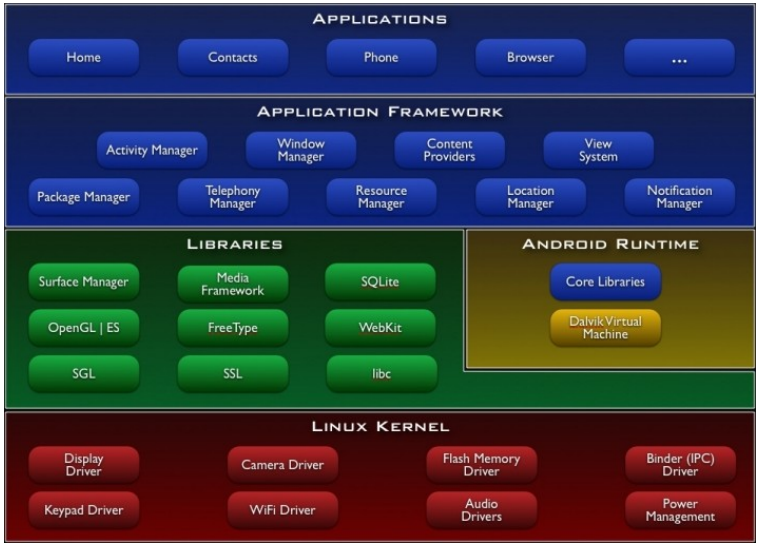
\includegraphics[scale=0.7]{arch_thebigpicture.png}
\end{center}
Studieremo a fondo le \textbf{applicazioni} e parte dell'\textbf{Android Runtime}. Le \textbf{libraries} sono largamente invisibili e il \textbf{linux kernel} è utile da sapere.
\section{Struttura}
\textit{Bottom -- Up}
\paragraph{Kernel Linux} Alla base di tutto c'è il \textbf{kernel Linux standard, senza personalizzazioni}. Gli \textbf{adattamenti} per la parte telefonica sono \textbf{eseguiti tramite moduli del kernel}. Come display driver, driver per la tastiera keypad, driver camera, wifi, memoria flash, audio, driver binder (IPC) che cura Inter-Process Communication (diversamente da socket e FIFO, che non andavano bene per Android. \textbf{Su Android non ci sono solo file, ma oggetti con metodi}, e FIFO/socket adatte per trasferire flussi di byte. Il \textbf{binder fa comunicare processi in termini object-oriented}). Per ultimo c'è il power management driver.\\
Per il resto è il kernel linux tanto conosciuto e amato: utenti, diritti, shell, librerie, thread e comandi.
\paragraph{Librerie} Librerie \texttt{.so}, che fanno tantissime cose. Tra esse ci sono: surface manager (equivalente dei window system X o wayland), OpenGL ES per la grafica 3D, FreeType, SSL (HTTPS e Secure Socket Layer), WebKit, SQLite, libc (scanf, strlen\ldots).
\subparagraph{Android Runtime} In aggiunta alle librerie, c'è anche la \textbf{Macchina Virtuale che esegue il codice delle applicazioni Android} (\textbf{Dalvik}/\textbf{ART}), insieme alle core libraries (garbage collector, heap, memoria\ldots)
\paragraph{Separazione tra mondo Java e mondo del codice eseguibile ARM} Da qui in poi c'è il linguaggio Java, fin'ora il linguaggio (del kernel linux) è il C.
\paragraph{Application Framework} S.O. rappresentato da oggetti nello heap. Librerie: package manager, telefony manager, activity manager, window manager, location manager (GPS), notification manager
\paragraph{Applicazioni} Tra cui servizi interni: home, contatti, telefono, browser\ldots Firmate a chiave asimmetrica. Platform key per applicazioni che usano funzioni critiche, chiave che firma il kernel.
\section{Dalvik}
\section{ART}
Android RunTime
\end{document}
